\documentclass[12pt]{softwaremanual}


\author{Joseph Schoonover}
\title{}
\date{}


\begin{document}

% Doing a custom title-page
\begin{titlingpage}
    
        \vspace*{2cm}
        
     \begin{flushright}
        {\fontfamily{cmss}\selectfont
        \HUGE{\textbf{ Spectral Element Method }}\\
        }
       
        \vspace{1cm}
        
        \huge{
        \textbf{
        \textit{
        \textcolor{blue}{
           Geometry
        }}}}
        
     \end{flushright}
         
        \vspace{2cm}
        
     \begin{center}
     
        %Do a subtitle here if you like
        {\fontfamily{cmss}\selectfont
        \huge{
           Software Manual
        }
        
        \vspace{1.5cm}
        
        % Enter the author's name
        \textbf{
        \large{
           \theauthor 
         }}}
        
        \vfill
        
        
        \vspace{0.8cm}
        
     \end{center}
        
    
\end{titlingpage}



\tableofcontents


\chapter{Purpose and Overview}
Spectral element methods are gaining popularity in the realm of geophysics. The Discontinuous Galerkin Spectral Element Method (DGSEM) is being applied in studies of earthquakes \textbf{(?)}, general ocean circulation through the shallow water equations \citep{Iskandarani1993} and hydrostatic primitive equations \citep{Iskandarani2000}. Additionally, the Continuous Galerkin Spectral Element Method (CGSEM) is being applied to elliptic and parabolic systems for studying topographic waves \citep{Schoonover2016}, \textit{and other phenomena}. These techniques are flexible in that the computational core of these algorithms are geometry independent, provided the physical domain is decomposed into an arrangement of quadrilateral (in 2-D) or hexahedral (3-D) spectral elements. Neither open-source nor propietary mesh generation software has met the needs of spectral mesh generation (at the time this document was written). The popularity of these methods for there use in problems with complicated geometry has motivated the development of a collection of data-structures, modules and programs to aid in the generation of spectral element meshes.

The purpose of the software described herein is two-fold : 
\begin{enumerate}
\item Provide the necessary data structures to store and query spectral element mesh information for is use in DG or CGSEM algorithms.
\item Use the data structures for developing an interactive mesh generation program which provides a suite of mesh quality checks.
\end{enumerate}
The latter of these two is part of a long term goal towards developing a self contained spectral element methods software package. Eventually, it would be ideal to port these Fortran modules with a Graphical User Interface which would allow for inuitive mesh generation.

The software design reflects the need for these data-structures in two different settings, namely, (1) mesh generation and (2) numerical computation. Because, each of the data structures which are used to define the mesh are offered in two flavors. 

For mesh generation, we prefer to have dynamic memory in the sense that inserting mesh primitives (e.g. nodes, edges, elements, etc.) should be allowed for. The user should not have to specify the number of mesh primitives a'priori; for an unstructured mesh, this is usually determined as a result of the mesh generation process. In this flavor of the data-structures and modules, we opt for the use of linked-lists which allow for easy and quick insertion of additional primitives. In the mesh generation process, generating and querying mesh information are the only tasks. A linked-list is not the most efficient structure for querying mesh information, but given that this is only one of two main tasks we prefer to give up efficiency in exchange for flexibility.

In conducting numerical computations with SEM, querying mesh information is a small part of the larger computations that is executed very often. Minimizing the time spent in obtaining mesh information is therefore crucial. In the numerical computation implementation of the geometry modules, we opt for arrays with fixed sizes, since arrays offer a much faster means of obtaining information. By the time the computation is being run, it is assumed that the mesh generation is complete, the number of mesh primitives is known and connectivity has already been established. 

The benefit of having these two flavors also allows for users to make use of either package in developing their own software. For those who work with a moving or adaptive mesh, the mesh generation implementation is likely the preferred structure to work with, given the ease in introducing new elements. The exchange in efficiency in the query process is made up for by a gain in accuracy in the approximate solution. 

In this way, the software structure offers flexible solutions to problems with complex geometry. 

\chapter{The Mesh}
A mesh can be decomposed into the basic constituents :
\begin{enumerate}
\item Nodes
\item Edges
\item Faces (3-D only)
\item Elements (can be 2-D or 3-D).
\end{enumerate}
Accompanying these constituents is the \textit{connectivity}. The connectivity describes what nodes make up each edge, what edges make up each face (in 3-D) or element (in 2-D), and establishes ``neighbor'' relationships among the elements. This chapter describes the data structures that are used to define the basic constituents of a mesh and outlines a set of accompanying procedures which are used to establish connectivity and handle file I/O of the spectral element mesh.
\begin{figure}[h!]
\begin{center}
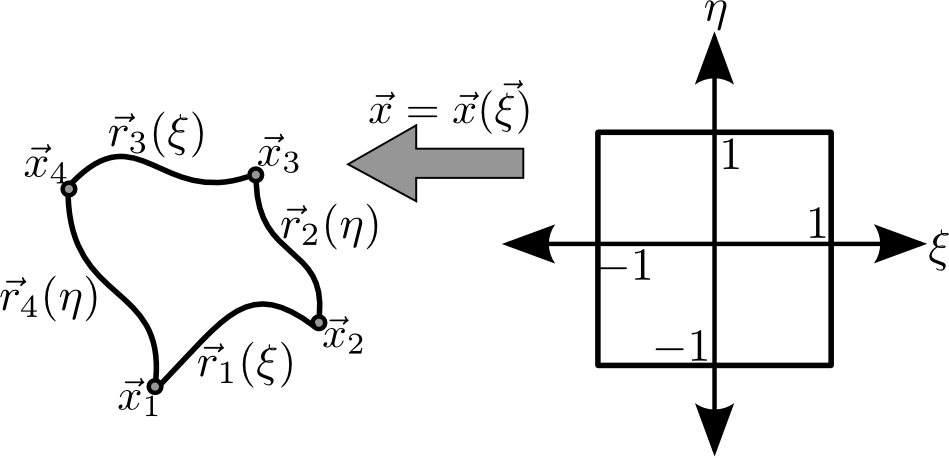
\includegraphics[scale=0.5]{figures/geometry/element2d.png}
\caption{An element in two-dimensions is illustrated which is described by four corner nodes, and its internal geometry is defined through the parametric curves which make up the edges and the use of transfinite interpolation.} \label{fig:element}
\end{center}
\end{figure}

Figure \ref{fig:element} depicts an element in two-dimensions which is described by its corner nodes and its internal geometry. The internal geometry, in this software, is generated using \textit{transfinite interpolation}.

\begin{figure}[h!]
\begin{center}
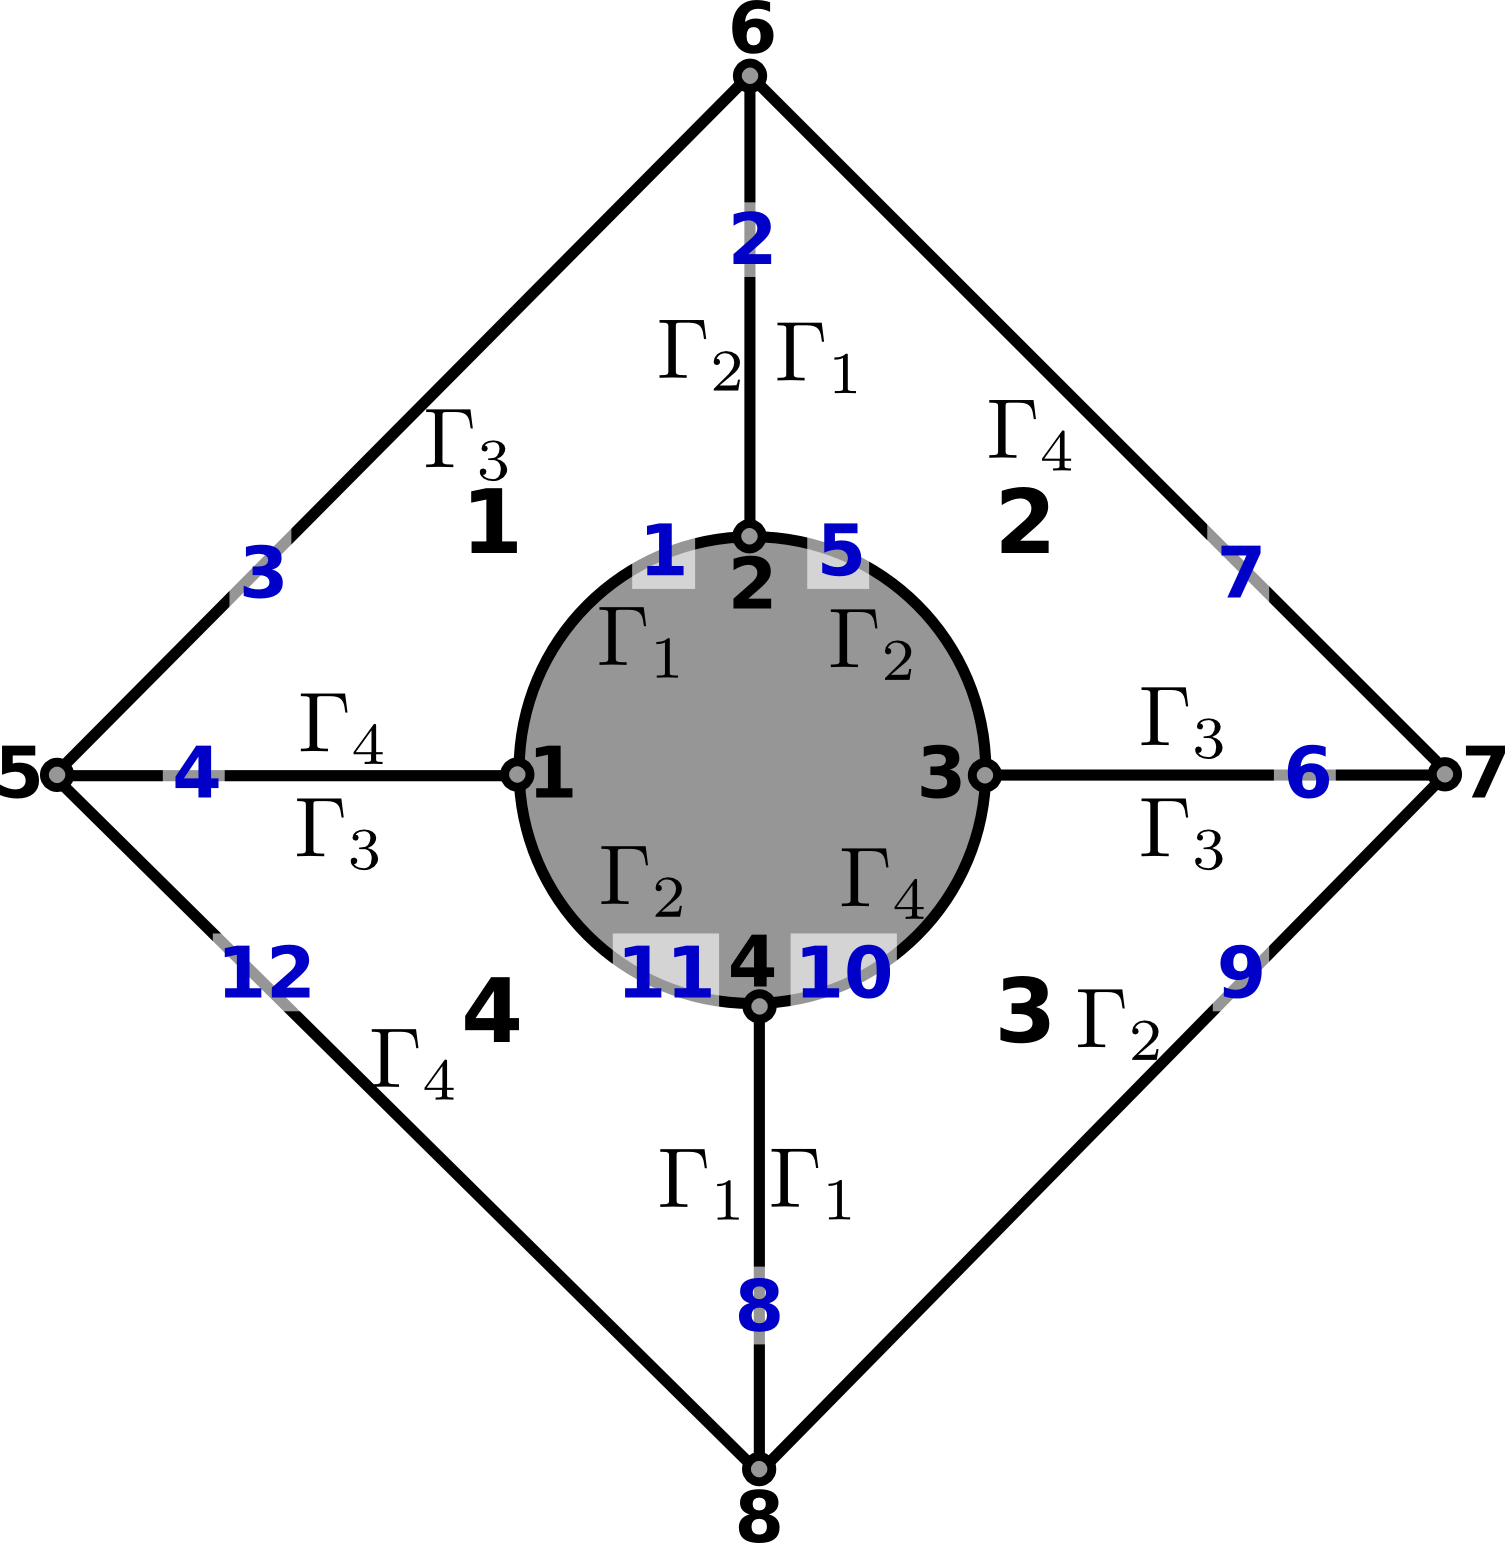
\includegraphics[scale=0.5]{figures/geometry/meshDepiction2D.png}
\caption{A simple mesh is shown which is composed of nodes, edges, and elements. } \label{fig:simplemesh}
\end{center}
\end{figure}


\begin{figure}[h!]
\begin{center}
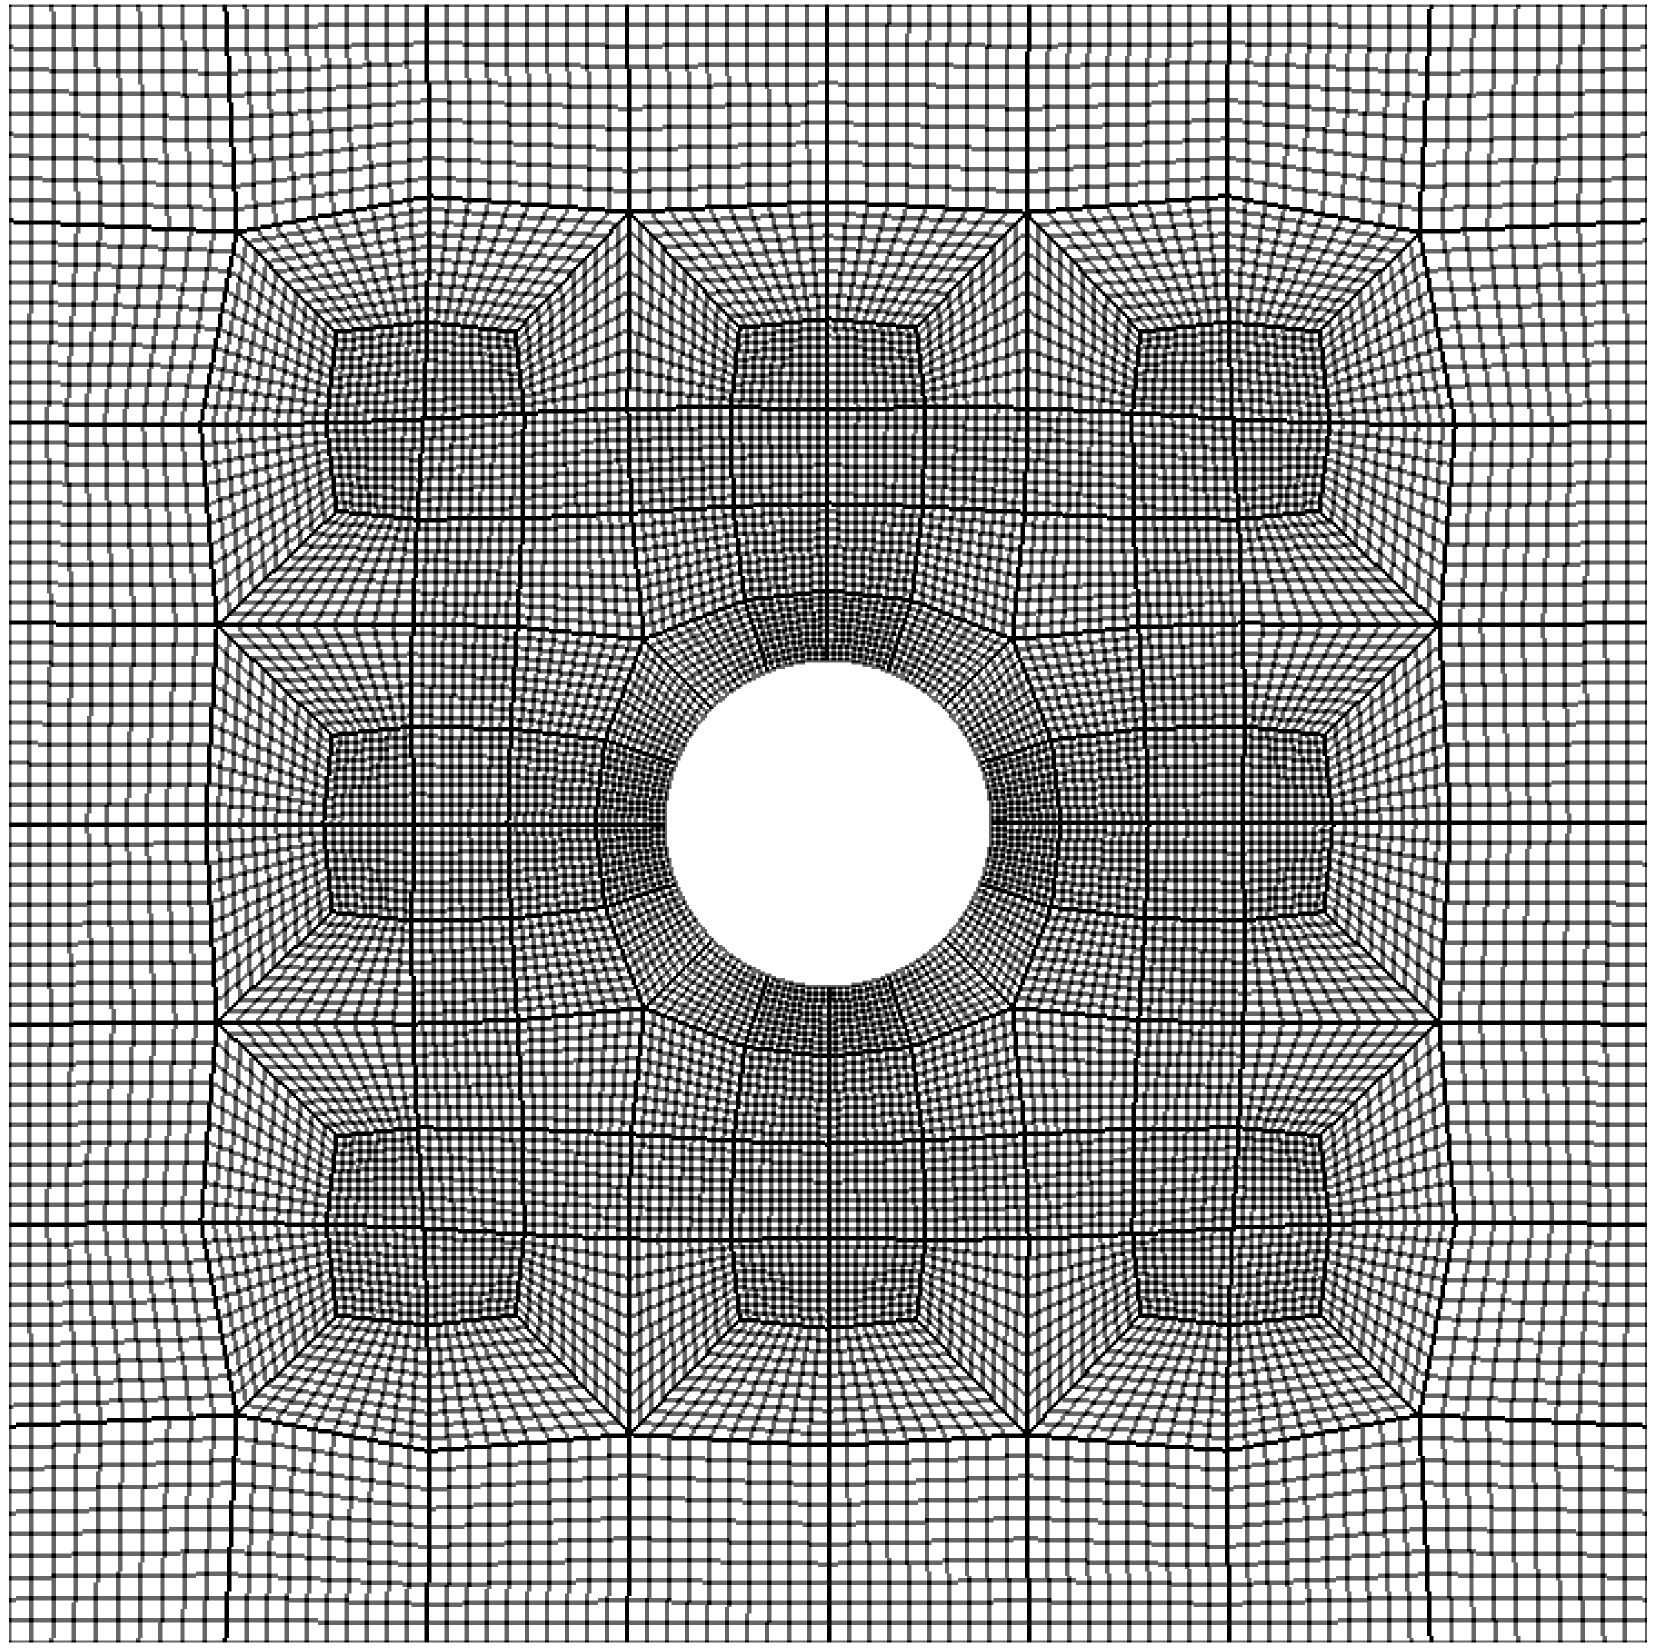
\includegraphics[scale=0.5]{figures/geometry/sample2dmesh.png}
\caption{A sample mesh is shown where each of the elements is outlined by the darker lines. The internal mesh is also shown with lighter colored lines. This particular mesh is generated with the SpecMesh software \citep{KoprivaSpecMesh} } \label{fig:samplemesh}
\end{center}
\end{figure}


\section{Data Structures and Routines}

  
\pagebreak
\bibliography{refs}
\bibliographystyle{plainnat}

\end{document}